%!TeX root=../solnQCQI.tex

\chapter{The quantum Fourier transform and its applications}

\Textbf{5.1} Give a direct proof that the linear transformation defined by Equation (5.2) is unitary.
$$\ket{j}\longrightarrow \sum_{k=0}^{N-1}e^{2\pi ijk/N}\ket{k}$$
\Soln First note that $e^{2\pi i/N}$ is an $N$-th root of unity, which we'll denote $\omega$.  The quantum Fourier transform (QFT) transforms $\ket{j}\rightarrow\sum_{k=0}^{N-1}\omega^{jk}\ket{k}$.  In matrix form:
$$QFT=\frac{1}{\sqrt{N}}\begin{bmatrix}1 & 1 & 1 & 1 &\ldots & 1 & 1 \\
1 & \omega^{1\cdot 1} & \omega^{2\cdot 1} & \omega^{3\cdot 1}& \ldots & \omega^{(N-2)\cdot 1} & \omega^{(N-1)\cdot 1} \\
1 & \omega^{1\cdot 2} & \omega^{2\cdot 2} & \omega^{3\cdot 2} & \ldots & \omega^{(N-2)\cdot 2} & \omega^{(N-1)\cdot 2} \\
1 & \omega^{1\cdot 3} & \omega^{2\cdot 3} & \omega^{3\cdot 3} & \ldots & \omega^{(N-2)\cdot 3} & \omega^{(N-1)\cdot 3} \\
\vdots & \vdots & \vdots & \vdots & \ddots & \vdots & \vdots \\
1 &  \omega^{1\cdot(N-2)} & \omega^{2\cdot (N-2)} & \omega^{3\cdot (N-2)} & \ldots & \omega^{(N-2)\cdot (N-2)} & \omega^{(N-1)\cdot (N-2)} \\
1 &  \omega^{1\cdot(N-1)} & \omega^{2\cdot (N-1)} & \omega^{3\cdot (N-1)} & \ldots & \omega^{(N-2)\cdot (N-1)} & \omega^{(N-1)\cdot (N-1)} \\
\end{bmatrix}$$
Noting that $\omega^* = \omega^{-1}$, we have
$$QFT^\dagger=\frac{1}{\sqrt{N}}\begin{bmatrix}1 & 1 & 1 & 1 &\ldots & 1 & 1 \\
1 & \omega^{-1\cdot 1} & \omega^{-1\cdot2} & \omega^{-1\cdot 3}& \ldots & \omega^{-1\cdot(N-2)} & \omega^{-1\cdot(N-1)} \\
1 & \omega^{-2\cdot1} & \omega^{-2\cdot 2} & \omega^{-2\cdot 3} & \ldots & \omega^{-2\cdot(N-2)} & \omega^{-2\cdot(N-1)} \\
1 & \omega^{-3\cdot1} & \omega^{-3\cdot2} & \omega^{-3\cdot 3} & \ldots &  \omega^{-3\cdot(N-2)} & \omega^{-3\cdot(N-1)} \\
\vdots & \vdots & \vdots & \vdots & \ddots & \vdots & \vdots \\
1 &  \omega^{-(N-2)\cdot 1} & \omega^{-(N-2)\cdot 2} & \omega^{-(N-2)\cdot 3} & \ldots & \omega^{-(N-2)\cdot (N-2)} & \omega^{-(N-2)\cdot (N-1)} \\
1 &  \omega^{-(N-1)\cdot 1} & \omega^{-(N-1)\cdot 2} & \omega^{-(N-1)\cdot 3} & \ldots & \omega^{-(N-1)\cdot (N-2)} & \omega^{-(N-1)\cdot (N-1)} \\
\end{bmatrix}$$
Now $QFT*QFT^\dagger=\frac{1}{N}\begin{bmatrix}\sum_{\ell=0}^{N-1} \omega^{\ell j}\omega^{-k\ell}\end{bmatrix}_{j,k} =\frac{1}{N} \begin{bmatrix}\sum_{\ell=0}^{N-1} \omega^{\ell (j-k)}\end{bmatrix}_{j,k}$.  When $j=k$, \textit{i.e.} on the diagonal, all exponents in the summation formula for the $j,k$ entry become 0, producing a sum of $N$ 1s, canceling the $\frac{1}{N}$ scalar and giving that the diagonal entries of $QFT*QFT^\dagger$ are all 1s.  For off-diagonal entries, \textit{i.e.} when $j\neq k$, let $a=j-k$.  Recognizing a finite geometric series and that $\omega$ is an $N$-th root of unity, we have:
$$\sum_{\ell=0}^{N-1} \omega^{\ell (j-k)} = \sum_{\ell=0}^{N-1} \omega^{a\cdot\ell} = 1+\omega^a+\omega^{2a}+\ldots+\omega^{(N-1)a} = \frac{1-\omega^{N\cdot a}}{1-\omega^a} = \frac{1-1^a}{1-\omega^a}= 0$$
Note that the denominator is non-zero, since $a\neq 0$.  Ultimately, $QFT*QFT^\dagger=I$, and $QFT$ is unitary.

\Textbf{5.2} Explicitly compute the Fourier transform of the $n$ qubit state $\ket{00\ldots0}$.
\Soln $QFT(\ket{00\ldots0})=\frac{1}{2^{n-1}}\sum_{k=0}^{\sqrt{2^n}}\ket{k}$.
\Textbf{5.3}
\Textbf{5.4} Give a decomposition of the controlled-$R_k$ gate into single qubit and \CNOT\ gates.
\Soln By Theorem 4.1 we may write $R_k=e^{i\alpha}R_z(\beta)R_y(\gamma)R_z(\delta)$ for some $\alpha, \beta, \gamma$ and $\delta$.  In this case, $\alpha=2\pi/2^{k+1}$, $\beta=0$, $\gamma=0$, and $\delta=2\pi/2^k$ suffice, since 
\begin{align*}
e^{2i\pi/2^{k+1}}R_z(0)R_y(0)R_z(2\pi/2^k)&=e^{2i\pi/2^{k+1}}I^2\begin{bmatrix}e^{-2i\pi/2^{k+1}} & 0 \\ 0 & e^{2i\pi/2^{k+1}}\end{bmatrix}
&=\begin{bmatrix}1 & 0 \\ 0 & e^{2i\pi/2^k}\end{bmatrix}=R_k\
\end{align*}
Following the proof of Corollary 4.2, set $A=R_z(0)R_y(0)=I, B=R_y(0)R_z(-2\pi/2^{k+1})=R_z(-2\pi/2^{k+1}),  C=R_z(2\pi/2^{k+1})$ so that $ABC=I$ and $U=e^{i\alpha}AXBXC$.  Applying the construction in Figure 4.6 gives:
\begin{center}
\begin{tikzpicture}[scale=1.000000,x=1pt,y=1pt]
\filldraw[color=white] (0.000000, -5.000000) rectangle (334.000000, 85.000000);
% Drawing wires
% Line 1: a1 W x_k
\draw[color=black] (0.000000,77.500000) -- (334.000000,77.500000);
\draw[color=black] (0.000000,77.500000) node[left] {$x_k$};
% Line 2: a2 W x_t
\draw[color=black] (0.000000,62.500000) -- (334.000000,62.500000);
\draw[color=black] (0.000000,62.500000) node[left] {$x_t$};
% Line 3: a3 W  breadth=50
\draw[color=black] (40.500000,30.000000) -- (334.000000,30.000000);
% Line 4: a4 W breadth=10
\draw[color=black] (40.500000,0.000000) -- (334.000000,0.000000);
% Done with wires; drawing gates
% Line 5: a2 G $R_k$ width=15
\begin{scope}
\draw[fill=white] (13.500000, 62.500000) +(-45.000000:10.606602pt and 8.485281pt) -- +(45.000000:10.606602pt and 8.485281pt) -- +(135.000000:10.606602pt and 8.485281pt) -- +(225.000000:10.606602pt and 8.485281pt) -- cycle;
\clip (13.500000, 62.500000) +(-45.000000:10.606602pt and 8.485281pt) -- +(45.000000:10.606602pt and 8.485281pt) -- +(135.000000:10.606602pt and 8.485281pt) -- +(225.000000:10.606602pt and 8.485281pt) -- cycle;
\draw (13.500000, 62.500000) node {$R_k$};
\end{scope}
% Line 7: a3 a4 =
\draw[fill=white,color=white] (6.000000, -6.000000) rectangle (21.000000, 36.000000);
\draw (13.500000, 15.000000) node {$=$};
% Line 6: a1 a2 =
\draw[fill=white,color=white] (33.000000, 56.500000) rectangle (48.000000, 83.500000);
\draw (40.500000, 70.000000) node {$=$};
% Line 8: a3 START
% Line 9: a4 START
% Line 10: a2 G $R_z(2\pi/2^{k+1})$ width=62
\begin{scope}
\draw[fill=white] (91.000000, 62.500000) +(-45.000000:43.840620pt and 8.485281pt) -- +(45.000000:43.840620pt and 8.485281pt) -- +(135.000000:43.840620pt and 8.485281pt) -- +(225.000000:43.840620pt and 8.485281pt) -- cycle;
\clip (91.000000, 62.500000) +(-45.000000:43.840620pt and 8.485281pt) -- +(45.000000:43.840620pt and 8.485281pt) -- +(135.000000:43.840620pt and 8.485281pt) -- +(225.000000:43.840620pt and 8.485281pt) -- cycle;
\draw (91.000000, 62.500000) node {$R_z(2\pi/2^{k+1})$};
\end{scope}
% Line 15: a4 G $R_z(2\pi/2^{k+1})$ width=62
\begin{scope}
\draw[fill=white] (91.000000, -0.000000) +(-45.000000:43.840620pt and 8.485281pt) -- +(45.000000:43.840620pt and 8.485281pt) -- +(135.000000:43.840620pt and 8.485281pt) -- +(225.000000:43.840620pt and 8.485281pt) -- cycle;
\clip (91.000000, -0.000000) +(-45.000000:43.840620pt and 8.485281pt) -- +(45.000000:43.840620pt and 8.485281pt) -- +(135.000000:43.840620pt and 8.485281pt) -- +(225.000000:43.840620pt and 8.485281pt) -- cycle;
\draw (91.000000, -0.000000) node {$R_z(2\pi/2^{k+1})$};
\end{scope}
% Line 11: a1 +a2
\draw (137.000000,77.500000) -- (137.000000,62.500000);
\filldraw (137.000000, 77.500000) circle(1.500000pt);
\begin{scope}
\draw[fill=white] (137.000000, 62.500000) circle(3.000000pt);
\clip (137.000000, 62.500000) circle(3.000000pt);
\draw (134.000000, 62.500000) -- (140.000000, 62.500000);
\draw (137.000000, 59.500000) -- (137.000000, 65.500000);
\end{scope}
% Line 16: a3 +a4
\draw (137.000000,30.000000) -- (137.000000,0.000000);
\filldraw (137.000000, 30.000000) circle(1.500000pt);
\begin{scope}
\draw[fill=white] (137.000000, 0.000000) circle(3.000000pt);
\clip (137.000000, 0.000000) circle(3.000000pt);
\draw (134.000000, 0.000000) -- (140.000000, 0.000000);
\draw (137.000000, -3.000000) -- (137.000000, 3.000000);
\end{scope}
% Line 12: a2 G $R_z(-2\pi/2^{k+1})$ width=71
\begin{scope}
\draw[fill=white] (187.500000, 62.500000) +(-45.000000:50.204581pt and 8.485281pt) -- +(45.000000:50.204581pt and 8.485281pt) -- +(135.000000:50.204581pt and 8.485281pt) -- +(225.000000:50.204581pt and 8.485281pt) -- cycle;
\clip (187.500000, 62.500000) +(-45.000000:50.204581pt and 8.485281pt) -- +(45.000000:50.204581pt and 8.485281pt) -- +(135.000000:50.204581pt and 8.485281pt) -- +(225.000000:50.204581pt and 8.485281pt) -- cycle;
\draw (187.500000, 62.500000) node {$R_z(-2\pi/2^{k+1})$};
\end{scope}
% Line 17: a4 G $R_z(-2\pi/2^{k+1})$ width=71
\begin{scope}
\draw[fill=white] (187.500000, -0.000000) +(-45.000000:50.204581pt and 8.485281pt) -- +(45.000000:50.204581pt and 8.485281pt) -- +(135.000000:50.204581pt and 8.485281pt) -- +(225.000000:50.204581pt and 8.485281pt) -- cycle;
\clip (187.500000, -0.000000) +(-45.000000:50.204581pt and 8.485281pt) -- +(45.000000:50.204581pt and 8.485281pt) -- +(135.000000:50.204581pt and 8.485281pt) -- +(225.000000:50.204581pt and 8.485281pt) -- cycle;
\draw (187.500000, -0.000000) node {$R_z(-2\pi/2^{k+1})$};
\end{scope}
% Line 13: a1 +a2
\draw (238.000000,77.500000) -- (238.000000,62.500000);
\filldraw (238.000000, 77.500000) circle(1.500000pt);
\begin{scope}
\draw[fill=white] (238.000000, 62.500000) circle(3.000000pt);
\clip (238.000000, 62.500000) circle(3.000000pt);
\draw (235.000000, 62.500000) -- (241.000000, 62.500000);
\draw (238.000000, 59.500000) -- (238.000000, 65.500000);
\end{scope}
% Line 18: a3 +a4
\draw (238.000000,30.000000) -- (238.000000,0.000000);
\filldraw (238.000000, 30.000000) circle(1.500000pt);
\begin{scope}
\draw[fill=white] (238.000000, 0.000000) circle(3.000000pt);
\clip (238.000000, 0.000000) circle(3.000000pt);
\draw (235.000000, 0.000000) -- (241.000000, 0.000000);
\draw (238.000000, -3.000000) -- (238.000000, 3.000000);
\end{scope}
% Line 14: a1 P $\alpha$
\begin{scope}
\draw[fill=white] (290.500000, 77.500000) circle(6.000000pt);
\clip (290.500000, 77.500000) circle(6.000000pt);
\draw (290.500000, 77.500000) node {$\alpha$};
\end{scope}
% Line 19: a3 G $\begin{bmatrix}1 & 0 \\ 0 & e^{2i\pi/2^{k+1}}\end{bmatrix}$ height=40 width=75
\begin{scope}
\draw[fill=white] (290.500000, 30.000000) +(-45.000000:53.033009pt and 28.284271pt) -- +(45.000000:53.033009pt and 28.284271pt) -- +(135.000000:53.033009pt and 28.284271pt) -- +(225.000000:53.033009pt and 28.284271pt) -- cycle;
\clip (290.500000, 30.000000) +(-45.000000:53.033009pt and 28.284271pt) -- +(45.000000:53.033009pt and 28.284271pt) -- +(135.000000:53.033009pt and 28.284271pt) -- +(225.000000:53.033009pt and 28.284271pt) -- cycle;
\draw (290.500000, 30.000000) node {$\begin{bmatrix}1 & 0 \\ 0 & e^{2i\pi/2^{k+1}}\end{bmatrix}$};
\end{scope}
% Done with gates; drawing ending labels
% Done with ending labels; drawing cut lines and comments
% Done with comments
\end{tikzpicture}
\end{center}
\Textbf{5.5} Give a quantum circuit to perform the inverse quantum Fourier transform.
\Soln The inverse quantum Fourier transform is the $QFT^\dagger$ transformation shown in Exercise 5.1.  For a fixed computational basis state $\ket{k}$, 
\begin{align*}
QFT^\dagger(\ket{k})&=\frac{1}{\sqrt{N}}\sum_{j=0}^{N-1}e^{-2\pi ijk/2^n}\ket{j} \\
&=\frac{\Bigl(\ket{0}+e^{-2\pi i0.k_n}\ket{1}\Bigr)\Bigl(\ket{0}+e^{-2\pi i0.k_{n-1}k_n}\ket{1}\Bigr)\cdots\Bigl(\ket{0}+e^{-2\pi i0.k_1k_2\ldots k_{n-1}k_n}\ket{1}\Bigr)}{\sqrt{N}}
\end{align*}
Using $R_\ell^{\dagger}=\begin{bmatrix}1 & 0 \\ 0 & e^{-2\pi i/2^{\ell}}\end{bmatrix}$ instead of $R_\ell$ in Figure 5.1 will implement $QFT^\dagger$.  It's verification is effectively identical to that of Figure 5.1 on page 219.  For completeness, the circuit is diagrammed here:

\begin{center}
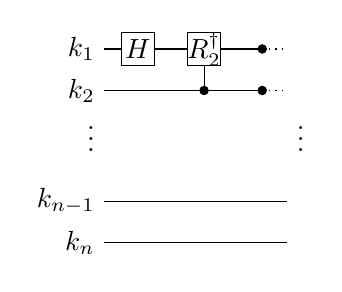
\begin{tikzpicture}[scale=1.000000,x=1pt,y=1pt]
\filldraw[color=white] (0.000000, -7.500000) rectangle (66.000000, 77.500000);
% Drawing wires
% Line 3: a1 W  \ket{k_1}
\draw[color=black] (0.000000,70.000000) -- (57.000000,70.000000);
\draw[color=black,dotted] (57.000000,70.000000) -- (66.000000,70.000000);
\draw[color=black] (0.000000,70.000000) node[left] {$\ket{k_1}$};
% Line 4: a2 W  \ket{k_2}
\draw[color=black] (0.000000,55.000000) -- (57.000000,55.000000);
\draw[color=black,dotted] (57.000000,55.000000) -- (66.000000,55.000000);
\draw[color=black] (0.000000,55.000000) node[left] {$\ket{k_2}$};
% Line 5: ...b W breadth=25
\draw[color=black] (0.000000,35.000000) node[anchor=mid east] {$\vdots$};
% Line 6: km W \ket{k_{n-1}}
\draw[color=black] (0.000000,15.000000) -- (66.000000,15.000000);
\draw[color=black] (0.000000,15.000000) node[left] {$\ket{k_{n-1}}$};
% Line 7: kn W \ket{k_n}
\draw[color=black] (0.000000,0.000000) -- (66.000000,0.000000);
\draw[color=black] (0.000000,0.000000) node[left] {$\ket{k_n}$};
% Done with wires; drawing gates
% Line 8: a1 H
\begin{scope}
\draw[fill=white] (12.000000, 70.000000) +(-45.000000:8.485281pt and 8.485281pt) -- +(45.000000:8.485281pt and 8.485281pt) -- +(135.000000:8.485281pt and 8.485281pt) -- +(225.000000:8.485281pt and 8.485281pt) -- cycle;
\clip (12.000000, 70.000000) +(-45.000000:8.485281pt and 8.485281pt) -- +(45.000000:8.485281pt and 8.485281pt) -- +(135.000000:8.485281pt and 8.485281pt) -- +(225.000000:8.485281pt and 8.485281pt) -- cycle;
\draw (12.000000, 70.000000) node {$H$};
\end{scope}
% Line 9: a1 G $R_2$ a2
\draw (36.000000,70.000000) -- (36.000000,55.000000);
\begin{scope}
\draw[fill=white] (36.000000, 70.000000) +(-45.000000:8.485281pt and 8.485281pt) -- +(45.000000:8.485281pt and 8.485281pt) -- +(135.000000:8.485281pt and 8.485281pt) -- +(225.000000:8.485281pt and 8.485281pt) -- cycle;
\clip (36.000000, 70.000000) +(-45.000000:8.485281pt and 8.485281pt) -- +(45.000000:8.485281pt and 8.485281pt) -- +(135.000000:8.485281pt and 8.485281pt) -- +(225.000000:8.485281pt and 8.485281pt) -- cycle;
\draw (36.000000, 70.000000) node {$R_2^\dagger$};
\end{scope}
\filldraw (36.000000, 55.000000) circle(1.500000pt);
% Line 10: a1:dot
\filldraw (57.000000, 70.000000) circle(1.500000pt);
% Line 11: a2:dot
\filldraw (57.000000, 55.000000) circle(1.500000pt);
% Done with gates; drawing ending labels
\draw[color=black] (66.000000,35.000000) node[anchor=mid west] {$\vdots$};
% Done with ending labels; drawing cut lines and comments
% Done with comments
\end{tikzpicture}
\end{center}

\Textbf{5.6} \textbf{(Approximate quantum Fourier transform)}  The quantum circuit construction of the quantum Fourier transform apparently requires gates of exponential precision in the number of qubits used.  However, such precision is never required in any quantum circuit of polynomial size.  For example, let $U$ be the ideal quantum Fourier transform on $n$ qubits, and $V$ be the transform which results if the controlled $R_k$ gates are performed to a precision of $\Delta = 1/p(n)$ for some polynomial $p(n)$.  Show that the error $E(U,V)=\max_{\ket{\psi}}\norm{(U-V)\ket{\psi}}$ scales as $\Theta(n^2/p(n))$, and thus polynomial precision in each gate is sufficient to guarantee polynomial accuracy in the output state.
\Soln 
Let $R^i_j$ be the controlled $R_j$ gate, controlled by the qubit with index $j$ in Figure 5.1 (1-up), targeting the qubit with index $i$.  Let $R'^i_j$ be the same gate performed with precision to a precision of $\Delta$.  Note that the superscripts indicate the target and are not exponents.
\begin{align*}
E(U,V) &\equiv \max_{\ket{\psi}}\norm{(U-V)\ket{\psi}} \tag{definition} \\
&= \max_{\ket{\psi}}\ \Bigl|\Bigl|(H^1R^1_2R^1_3\cdots R^1_n H^2R^2_2\cdots R^2_{n-1}\cdots H^{n-1}R^{n-1}_2 H^n \\
&\ \ \ \ \ \ \ \ \ \ \ -H^1R'^1_2R'^1_3\cdots R'^1_n H^2R'^2_2\cdots R'^2_{n-1}\cdots H^{n-1}R'^{n-1}_2 H^n)\ket{\psi}\Bigr|\Bigr|
\end{align*}
The trick seems to be to apply a (supposedly true) lemma that $E(AB,A'B') \leq E(A,A')+E(B,B')$. This doesn't seem to be entirely obvious, but if allowed to apply it:
\begin{align*}
&\leq E(H^1, H^1) + E(R_2^1,R'^1_2) + \ldots + E(R_n^1, R'^1_n) + E(H^2, H^2) \\
&\ \ \ \ + E(R_2^2,R'^2_2) + \ldots + E(R_{n-1}^2, R'^2_{n-1}) +\ldots \\
&\ \ \ \ + E(H^{n-1}, H^{n-1}) + E(R^{n-1}_2, R'^{n-1}_2) + E(H^n,H^n) \\
&\leq 0+\Delta + \ldots + \Delta + 0 + \Delta +\ldots + \Delta + \ldots + 0 + \Delta + 0 \\
&= (n-1)\Delta + (n-2)\Delta + \ldots + \Delta \\
&= \Delta\sum_{i=1}^{n-1} i \\
&= \left(\frac{n(n-1)}{2}\right)\delta \leq \frac{n*(n-1)}{2p(n)} = O(n^2/p(n))
\end{align*}
This only gives an upper bound.  A lower bound is less important and would seem to require a lower bound in the lemma, which I'm suspicious of.  It would also require the assumption that the controlled $R_k$ gates are performed with causal error $\Delta$.  In practice, this is unlikely to be the case.  In application, the only causal errors are likely to be the result of simply not performing the controlled-$R_k$ gates at all, for $k$ above some fixed threshold.  Doing so would introduce causal errors, but those errors would depend on $k$, not $n$. The threshold for $k$ may depend on $n$, and the \textit{total} error depends on the number of controlled-$R_k$ gates not performed which is determined by $n$, but individually the error in not performing a single controlled-$R_k$ would depend only on $k$.

\Textbf{5.7} Additional insight into the circuit in Figure 5.2 amy be obtained by showing, as you should now do, that the effect of the sequence of controlled-$U$ operations like that in Figure 5.2 is to take the state $\ket{j}\ket{u}$ to $\ket{j}U^j\ket{u}$. (Note that this does not depend on $\ket{u}$ being an eigenstate of $U$.
\Soln Note that $\ket{j}$ is implicitly assumed to be a computational basis state, so let's write $j = j_{t-1}j_{t-2}\ldots j_1j_0$ in binary.  Preferring to write quantum registers in big-endian: $\ket{j}=\ket{j_0j_1\ldots j_{t-2}j_{t-1}}$.  The sequence of controlled-$U$ gates is thus:
\begin{center}
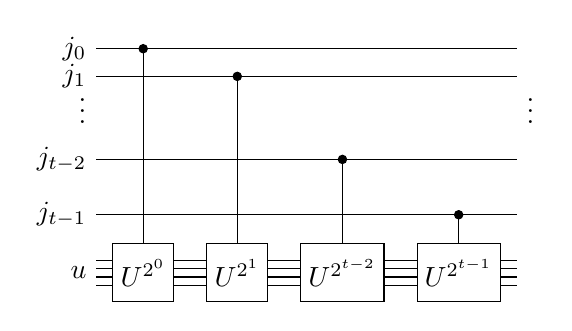
\begin{tikzpicture}[scale=1.000000,x=1pt,y=1pt]
\filldraw[color=white] (0.000000, -1.500000) rectangle (152.000000, 90.500000);
% Drawing wires
% Line 1: a0 W \ket{j_0} breadth=10
\draw[color=black] (0.000000,85.500000) -- (152.000000,85.500000);
\draw[color=black] (0.000000,85.500000) node[left] {$\ket{j_0}$};
% Line 2: a1 W \ket{j_1} breadth=10
\draw[color=black] (0.000000,75.500000) -- (152.000000,75.500000);
\draw[color=black] (0.000000,75.500000) node[left] {$\ket{j_1}$};
% Line 3: ...b W breadth=20
\draw[color=black] (0.000000,60.500000) node[anchor=mid east] {$\vdots$};
% Line 4: at2 W \ket{j_{t-2}} breadth=10
\draw[color=black] (0.000000,45.500000) -- (152.000000,45.500000);
\draw[color=black] (0.000000,45.500000) node[left] {$\ket{j_{t-2}}$};
% Line 5: at1 W \ket{j_{t-1}} breadth=30
\draw[color=black] (0.000000,25.500000) -- (152.000000,25.500000);
\draw[color=black] (0.000000,25.500000) node[left] {$\ket{j_{t-1}}$};
% Line 6: t1 t2 t3 t4 W \ket{u} breadth=3
\draw[color=black] (0.000000,9.000000) -- (152.000000,9.000000);
%   Deferring wire label at (0.000000,9.000000)
% Line 6: t1 t2 t3 t4 W \ket{u} breadth=3
\draw[color=black] (0.000000,6.000000) -- (152.000000,6.000000);
%   Deferring wire label at (0.000000,6.000000)
% Line 6: t1 t2 t3 t4 W \ket{u} breadth=3
\draw[color=black] (0.000000,3.000000) -- (152.000000,3.000000);
%   Deferring wire label at (0.000000,3.000000)
% Line 6: t1 t2 t3 t4 W \ket{u} breadth=3
\draw[color=black] (0.000000,0.000000) -- (152.000000,0.000000);
\draw[color=black] (0.000000,4.500000) node[left] {$\ket{u}$};
% Done with wires; drawing gates
% Line 7: t1 t2 t3 t4 G $U^{2^0}$ a0 width=22 height=16
\draw (17.000000,85.500000) -- (17.000000,0.000000);
\begin{scope}
\draw[fill=white] (17.000000, 4.500000) +(-45.000000:15.556349pt and 14.849242pt) -- +(45.000000:15.556349pt and 14.849242pt) -- +(135.000000:15.556349pt and 14.849242pt) -- +(225.000000:15.556349pt and 14.849242pt) -- cycle;
\clip (17.000000, 4.500000) +(-45.000000:15.556349pt and 14.849242pt) -- +(45.000000:15.556349pt and 14.849242pt) -- +(135.000000:15.556349pt and 14.849242pt) -- +(225.000000:15.556349pt and 14.849242pt) -- cycle;
\draw (17.000000, 4.500000) node {$U^{2^0}$};
\end{scope}
\filldraw (17.000000, 85.500000) circle(1.500000pt);
% Line 8: t1 t2 t3 t4 G $U^{2^1}$ a1 width=22 height=16
\draw (51.000000,75.500000) -- (51.000000,0.000000);
\begin{scope}
\draw[fill=white] (51.000000, 4.500000) +(-45.000000:15.556349pt and 14.849242pt) -- +(45.000000:15.556349pt and 14.849242pt) -- +(135.000000:15.556349pt and 14.849242pt) -- +(225.000000:15.556349pt and 14.849242pt) -- cycle;
\clip (51.000000, 4.500000) +(-45.000000:15.556349pt and 14.849242pt) -- +(45.000000:15.556349pt and 14.849242pt) -- +(135.000000:15.556349pt and 14.849242pt) -- +(225.000000:15.556349pt and 14.849242pt) -- cycle;
\draw (51.000000, 4.500000) node {$U^{2^1}$};
\end{scope}
\filldraw (51.000000, 75.500000) circle(1.500000pt);
% Line 9: t1 t2 t3 t4 G $U^{2^{t-2}}$ at2 width=30 height=16
\draw (89.000000,45.500000) -- (89.000000,0.000000);
\begin{scope}
\draw[fill=white] (89.000000, 4.500000) +(-45.000000:21.213203pt and 14.849242pt) -- +(45.000000:21.213203pt and 14.849242pt) -- +(135.000000:21.213203pt and 14.849242pt) -- +(225.000000:21.213203pt and 14.849242pt) -- cycle;
\clip (89.000000, 4.500000) +(-45.000000:21.213203pt and 14.849242pt) -- +(45.000000:21.213203pt and 14.849242pt) -- +(135.000000:21.213203pt and 14.849242pt) -- +(225.000000:21.213203pt and 14.849242pt) -- cycle;
\draw (89.000000, 4.500000) node {$U^{2^{t-2}}$};
\end{scope}
\filldraw (89.000000, 45.500000) circle(1.500000pt);
% Line 10: t1 t2 t3 t4 G $U^{2^{t-1}}$ at1 width=30 height=16
\draw (131.000000,25.500000) -- (131.000000,0.000000);
\begin{scope}
\draw[fill=white] (131.000000, 4.500000) +(-45.000000:21.213203pt and 14.849242pt) -- +(45.000000:21.213203pt and 14.849242pt) -- +(135.000000:21.213203pt and 14.849242pt) -- +(225.000000:21.213203pt and 14.849242pt) -- cycle;
\clip (131.000000, 4.500000) +(-45.000000:21.213203pt and 14.849242pt) -- +(45.000000:21.213203pt and 14.849242pt) -- +(135.000000:21.213203pt and 14.849242pt) -- +(225.000000:21.213203pt and 14.849242pt) -- cycle;
\draw (131.000000, 4.500000) node {$U^{2^{t-1}}$};
\end{scope}
\filldraw (131.000000, 25.500000) circle(1.500000pt);
% Done with gates; drawing ending labels
\draw[color=black] (152.000000,60.500000) node[anchor=mid west] {$\vdots$};
% Done with ending labels; drawing cut lines and comments
% Done with comments
\end{tikzpicture}
\end{center}
with each $\ket{j_s}$ being either $\ket{0}$ or $\ket{1}$.  The controlled $U^{2^s}$ gate is applied to $\ket{u}$ if and only if $\ket{j_s} = \ket{1}$ which can be represented by multiplication of $\ket{u}$ by $U^{j_s2^s}$.
\begin{align*}
\ket{j}\ket{u} &= \ket{j_0j_1\ldots j_{t-2}j_{t-1}}\ket{u} \\
&\rightarrow \ket{j_0j_1\ldots j_{t-2}j_{t-1}}  U^{j_{t-1}2^{t-1}}U^{j_{t-2}2^{t-2}}\cdots U^{j_12^1}U^{j_02^0}\ket{u}\\
&= \ket{j_0j_1\ldots j_{t-2}j_{t-1}} U^{j_0j_1\ldots j_{t-2}j_{t-1}}\ket{u}  \tag{collect powers of $U$ in binary}\\
&= \ket{j}U^j\ket{u} \tag{recognize binary representation of $j$}
\end{align*}

\Textbf{5.8} Suppose the phase estimation algorithm takes the state $\ket{0}\ket{u}$ to the state $\ket{\widetilde{\varphi_u}}\ket{u}$, so that given then input $\ket{0}(\sum_uc_u\ket{u})$, the algorithm outputs $\sum_uc_u\ket{\widetilde{\varphi_u}}\ket{u}$.  Show that is $t$ is chosen according to (5.35), then the probability for measuring $\varphi_u$ accurate to $n$ bits at the conclusion of the phase estimation algorithm is at least $|c_u|^2(1-\epsilon)$.
\Soln Note that in this problem we assume $\{\ket{u}\}$ forms an eigenbasis, but that the bound on probability is requested for measuring $\varphi_u$ for some fixed eigenvalue, say $\upsilon$.  Measurement of the second register collapses the state  to $\ket{\widetilde\varphi_{\upsilon}}\ket{\upsilon}$ with probabily $|c_{\upsilon}|^2$, from which we can determine $\varphi_{\upsilon}$ accurate to $n$ bits with probability $1-\epsilon$.  Multiplying probabilities gives that performing phase estimation on $\ket{0}(\sum_uc_u\ket{u})$ gives a probability of measuring $\varphi_{\upsilon}$ accurate to $n$ bits of $|c_\upsilon|^2(1-\epsilon)$. 

\Textbf{5.9}
\Textbf{5.10} Show that the (multiplicative) order of $(x=)5$ mod $(N=)21$ is $6$.
\Soln It suffices to show that $5^t \not\equiv 1 \pmod{21}$ for $1\leq t < 5$, and that $5^6 \equiv 1 \pmod{21}$
\begin{center}
\begin{tabular}{|c|c|}
\hline
$t$ & $5^t \pmod{21}$ \\
\hline
\hline
0 & 1 \\
\hline
1 & 5 \\
\hline
2 & 4 \\
\hline
3 & 20 $(\equiv -1)$ \\
\hline
4 & 16 $(\equiv -5)$ \\
\hline
5 & 17 $(\equiv -4)$ \\
\hline
\hline
6 & 1 $(\equiv -20)$ \\
\hline
\end{tabular}
\end{center}

\Textbf{5.11} Show that the (multiplicative) order of $x$ (mod $N$) satisfies $r \leq N$.
\Soln Note that $x\neq 0$, since $0^r \equiv 0 \pmod{N}$ for all $r$, and the order of $1$ is $1$ for all $N$.  For $N\geq 2$, see Euler's totient theorem which states that when $\gcd(x,N)=1$, $x^{\phi(N)}\equiv 1 \pmod{N}$, where $\phi(N)$ is the totient of $N$, \textit{i.e.} the number of integers $1\leq n \leq N$ such that $\gcd(n,N) = 1$.  For $N\geq 2$, $\gcd(N,N) \neq 1$, so $\phi(N) \leq N-1$.  Equality holds (for $\phi$ and the order of $x$) if and only if $N$ is prime.  In the end, for $N \geq 2$, the order of any integer $x$ comprime to the modulus $N$ is at most $\phi(N) \leq N-1$.  Note, with a little additional consideration it can be shown that the order of $x$ is, in fact, a divisor $\phi(N)$ by using Lagrange's Theorem on subgroup orders applied to the cyclic group generated by $x$ in the multiplicative group mod $N$.

\Textbf{5.12} Show that $U$ is unitary (\textit{Hint:} $x$ is co-prime to $N$, and therefore has an inverse modulo $N$)
\Soln $U$ performs modular multiplication by $x$.  When $x$ is coprime to $N$, modular multiplication by $x$ executes a permutation of the computational basis states, that is, $U$ is a permutation matrix.  Inverses of permutation matrices are easily seen to be their transposes.  So, $U^\dagger U = U^TU = U^{-1}U = I$, and $U$ is unitary.

\Textbf{5.13} Prove (5.44): $$\frac{1}{\sqrt{r}}\sum_{s=0}^{r-1}\ket{u_s} = \ket{1}.$$ (\textit{Hint:} $\sum_{s=0}^{r-1}\exp(-2\pi isk/r) = r\delta_{k0}$.)  In fact, prove that $$\frac{1}{\sqrt{r}}\sum_{s=0}^{r-1}e^{2\pi isk/r}\ket{u_s} = \ket{x^k\hspace{-10pt}\pmod{N}}.$$
\Soln Note that in this exercise $k$ is fixed, whereas in the definition of $\ket{u_s}$ in equation (5.37), $k$ is an index that is iterated over.  Below, we'll iterate over $k'$ instead of $k$.  In the hint, $k$ is arbitrary.  We'll apply it to $(k-k')$ at a point at which $k'$ will also be fixed, yielding $\sum_{s=0}^{r-1}\exp(-2\pi is(k-k')/r) = r\delta_{(k-k')0}=r\delta_{kk'}$.
\begin{align*}
\frac{1}{\sqrt{r}}\sum_{s=0}^{r-1}e^{2\pi isk/r}\ket{u_s} &= \frac{1}{\sqrt{r}}\sum_{s=0}^{r-1}e^{2\pi isk/r}\left(\frac{1}{\sqrt{r}}\sum_{k'=0}^{r-1}e^{-2\pi isk'/r}\ket{x^{k'}\hspace{-10pt}\pmod{N}}\right)\\
&= \frac{1}{r}\sum_{s=0}^{r-1}\sum_{k'=0}^{r-1}e^{2\pi is(k-k')/r}\ket{x^{k'}\hspace{-10pt}\pmod{N}} \tag{distribute} \\
&= \frac{1}{r}\sum_{k'=0}^{r-1}\left(\sum_{s=0}^{r-1}e^{2\pi is(k-k')/r}\right)\ket{x^{k'}\hspace{-10pt}\pmod{N}} \tag{change order} \\
&= \frac{1}{r}\sum_{k'=0}^{r-1}r\delta_{kk'}\ket{x^{k'}\hspace{-10pt}\pmod{N}} \tag{apply hint} \\
&= \ket{x^{k}\hspace{-10pt}\pmod{N}} \tag{collect non-zero terms}
\end{align*}

\Textbf{5.14} The quantum state produced in the order-finding algorithm, before the inverse Fourier transform, is $$\ket{\psi} = \sum_{j=0}^{2^t-1}\ket{j}U^j\ket{1} = \sum_{j=0}^{2^t-1}\ket{j}\ket{x^j\hspace{-10pt}\pmod{N}},$$ if we initialize the second register as $\ket{1}$.  Show that the same state is obtained if we replace $U^j$ with a \textit{different} unitary transform $V$, which computes $$V\ket{j}{\ket{k}} = \ket{j}\ket{k+x^j\hspace{-10pt}\pmod{N}},$$ and start the second register in the state $\ket{0}$.  Also show how to construct $V$ in $O(L^3)$ gates.
\Soln Initializing the second register in the state $\ket{k} = \ket{0}$ means that applying $V$ produces $$V\left(\sum_{j=0}^{2^t-1}\ket{j}\ket{0}\right) = \sum_{j=0}^{2^t-1}V\ket{j}\ket{0} = \sum_{j=0}^{2^t-1}\ket{j}\ket{0+x^j\pmod{N}} = \sum_{j=0}^{2^t-1}\ket{j}\ket{x^j\pmod{N}}.$$  This might be missing the point, but if explicitly required, $V$ can be implemented by first applying $U$ to $\ket{j}\ket{1}\ket{k}$ to produce the state $\ket{j}\ket{x^j\pmod{N}}\ket{0}$, where the $\ket{k}$ is the state of a third register whose length is the same as the second.  Then, adding the second register to the third $\pmod{N}$ produces $\ket{j}\ket{x^j\pmod{N}}\ket{x^j\pmod{N}}$.  Modular addition can be performed using $O(L)$ gates, so the complexity of $V$ can be seen to be $O(L^3+L)=O(L^3)$.

\Textbf{5.15} Show that the least common multiple of positive integers $x$ and $y$ is $xy/\gcd(x,y)$, and thus may be computed in $O(L^2)$ operations if $x$ and $y$ are $L$ bit numbers.
\Soln This is trivial ... still, note that $\gcd(x,y) | x$ and $\gcd(x,y) | y$, so $x = k\gcd(x,y)$ and $y=\ell\gcd(x,y)$ for some $k$ and $\ell$.  Now $xy/\gcd(x,y) = x\ell = ky$, so $xy/\gcd(x,y)$ is a common multiple of $x$ and $y$. To show it is the least common multiple, it is most instructive to rely on the unique prime factorization formula, but instead, note that by the Euclidean algorithm (or Bezout's Lemma), there exists integers $a$ and $b$ such that $\gcd(x,y) = ax+by$ (one of $a$ and $b$ is negative).  Let $m$ be any common multiple, meaning $m=\kappa x=\lambda y$.  Now $m\gcd(x,y)=max+mby=\lambda yax + \kappa xby = xy(\lambda a + \kappa b)$. Now $xy$ is divisible by $\gcd(x,y)$ by definition, so we can write $m = \frac{xy}{\gcd(x,y)}(\lambda a + \kappa b)$, and $\frac{xy}{\gcd(x,y)}$ divides $m$. So, $m$ cannot be the least common multiple, unless $m$ is itself $\frac{xy}{\gcd(x,y)}$.

The complexity of classical (schoolbook) multiplication and division are both $O(L^2)$.  The complexity of calculating the gcd is at most $O(L^2)$ so that in total the least common multiple can be calculated in $O(L^2)$ operations.

\Textbf{5.16} For all $x\geq 2$ prove that $\int_{x}^{x+1}1/y^2dy \geq 2/3x^2$.  Show that $$\sum_q \frac{1}{q^2} \leq \frac{3}{2}\int_{2}^{\infty}\frac{1}{y^2}dy = 3/4,$$ and thus that (5.58) holds.
\Soln $\int_{x}^{x+1}1/y^2dy = \frac{-1}{y}\Big|_{x}^{x+1} = \frac{1}{x}-\frac{1}{x+1} = \frac{1}{x(x+1)}$.  for $x\geq 2$, note that both $x$ and $(x-2)$ are positive, so that
\begin{align*}
0 &\leq x(x-2) \tag{by assumption} \\
 &= x^2-2x \\
2x^2+2x &\leq 3x^2 \tag{add $2x^2+2x$ to both sides} \\
2/3x^2 &\leq 1/(x^2+x) \tag{multiply by $1/(3x^2)(x^2+x)$, note: its positive} \\
 &= \int_{x}^{x+1}1/y^2dy
 \end{align*}
 So $\int_x^{x+1}1/y^2dy \geq 2/3x^2$, or more applicably, $\frac{1}{x^2} \leq \frac{3}{2}\int_x^{x+1}\frac{1}{y^2}dy$.  For the second part:
 $$\sum_{q\ \mathrm{prime}}\frac{1}{q^2} < \sum_{x=2}^{\infty} \frac{1}{x^2} \leq \sum_{x=2}^\infty\frac{3}{2}\int_x^{x+1}\frac{1}{y^2}dy = \int_2^\infty\frac{1}{y^2}dy = \left.\frac{-3}{2y}\right\rvert^\infty_2 = \frac{3}{4}.$$  Using this bound for the sum of prime square reciprocals in equation 5.57 gives the lower bound on probability in equation 5.58.  This bound is quite loose though.  The prime square reciprocal sum has been studies extensively.  Summing over all integers, not just primes, we can apply the solution (due to Euler) to the Basel problem:
 $$\sum_{q\ \mathrm{prime}} \frac{1}{q^2} \leq -1 + \sum_{x=1}^\infty \frac{1}{x^2} = -1 +\frac{\pi^2}{6} \approx 0.6450$$.  Euler also evaluated the sum over primes specifically to high precision.  See page 480 of \url{http://www.17centurymaths.com/contents/euler/introductiontoanalysisvolone/ch15vol1.pdf}
 $$\sum_{q\ \mathrm{prime}}\frac{1}{q^2} \approx 0.45225.$$
 
\Textbf{5.17} Suppose $N$ is $L$ bits long.  The aim of this exercise is to find an efficient classical algorithm to determine whether $N=a^b$ for some integers $a \geq {\color{red}2}$ and $b \geq {\color{red}2}$.  This may be done as follows:
\begin{enumerate}[label=(\arabic*)]
\item Show that $b$, if it exists, satisfies $b\leq L$.
\item Show that it takes at most $O(L^2)$ operations to compute $\log_2 N, x=y/b$ for $b\leq L$, and the two integers $u_1$ and $u_2$ nearest to $2^x$.
\item Show that it takes at most $O(L^2)$ operations to compute $u_1^b$ and $u_2^b$ (use repeated squaring) and check to see if either is equal to $N$.
\item Combine the previous results to give an $O(L^3)$ operation algorithm to dtermine whether $N=a^b$ for integers $a$ and $b$.
\end{enumerate}
\Soln
\begin{enumerate}[label=(\arabic*)]
\item In fact, $b \leq L-1$.  By assumption $a^b = N$, so $b = \log_a N = \log_2 N/\log_2 a \leq \log_2 N \leq \lceil \log_2 N\rceil \equiv L$.  Being integers, $b \leq L - 1$ unless equality holds throughout.  Equality can hold only if $a=2$ and $\log_2 N$ is an integer, \textit{i.e} $N=2^b$, but in this case $L=b+1$, so once again $b \leq L-1$.  In (2) and (3) below, we'll assume $b$ is fixed. The result will be that algorithm generated actually has complexity $O(L^4)$.  If for fixed $a$ the value of $b$ can be determined without iteration, such as during the sequence of square and (maybe) multiply operations constructing $u_1^b$ and $u_2^b$ described in (3), then this might reduce the complexity to $O(L^3)$.
\item Note, we don't need $\log_2 N$ as a decimal number, we actually need $\lceil \log_2 N\rceil$.  To calculate this, start with 1 and iteratively double by adding the result to itself until it is at least $N$.  Doing so requires $L$ iterations, each of which consists of a single standard schoolbook addition and an integer comparison, both of which can be done in $O(L)$ steps, so that in total calculating $\lceil \log_2 N\rceil$ requires $L*O(L)=O(L^2)$ steps.  [Note: one additional comparison might be required to initialize (or terminate) the algorithm, but this will not change the asymptotics.]  I don't know what $y$ is, but it must be a fixed $L$-bit value ($y\leq N-1$).  Schoolbook division of one $L$-bit integer by another is well-known to have complexity $O(L^2)$.  The result, $x$, will be another $L$-bit integer at most $N-1$.  We construct $2^x$ by summing various powers of $2$.  Calculating $2^{2^i}$ can be done iteratively with the same sequence of $O(L)$ doublings described above.  Then $2^x$ can be assembled by adding the at most $O(L)$ powers of $2$ corresponding to the 1's in the binary representation of $x$.  Computing the binary representation of $x$ (in reverse order) can be done with an iterative sequence of $O(L)$ subtractions of the largest powers of 2 smaller than the current value (which can be determined with at most $O(L^2)$ comparisons).  The $O(L)$ subtractions, each requiring $O(L)$ operations, take at total of $O(L^2)$ operations.  $u_1$ and $u_2$ can be computed by adding and subtracting 1, taking $O(L)$ steps each.  So, all requested operations can be performed in $O(L^2)$ steps.
\item Calculating $u_1^b$ and $u_2^b$ can be done in $O(L^2)$ steps similar to the calculation of $2^x$ above, but instead of adding powers of 2 specified by the binary representation of $x$, we square, or square and multiply according the binary representation of $b$.  The binary representation of $b$ can be calculated in $O(L^2)$ steps, as described for $x$ above.  Then, start with $z=u_i$ ($i=1,2$).  For each bit except the most significant (in order from least significant to second-most significant), square $z$ and if the bit of $b$ is a 1, multiply by $u_i$.  Using comparisons (with complexity $O(L)$) we can decide to stop when the result is at least $N$ and test for equality if we've completed the exponentiation.   Squaring doubles the bitlength of the result, so lets assume we perform $\ell$ squarings.  Note that $\ell \leq \log_2 L$.  Then $u_i$ must have had at most $L/2^\ell$ bits.  After the $j$-th square and (maybe) multiply operation, the result has at most $L/2^{\ell-j}$ bits.  In the next step, the square and multiply each require $O((L/2^{\ell-j})^2)$ steps.  Over all $\ell$ iterations, $\sum_{j=0}^{\ell-1} O((L/2^{\ell-j})^2)= O(L^2 \cdot \sum_{j=1}^\ell 1/2^{2j})= O(\frac{1}{3} L^2) = O(L^2)$ operations are required to perform the square and (maybe) multiplies (where the additional 1/3 constant is the value of the infinite geometric series as opposed to the finite).  Adding the comparisons with $N$ contributes only $O(\ell L)= O(L\log_2 L)=O(L^2)$ (where here, equality indicates set-containment, not complexity class equality). So, in the end, for fixed $b$, calculating $u_i^b$ and testing whether either is equal to $N$ requires only $O(L^2)$ operations.
\item The final step in the $O(L^4)$ algorithm to determine if $N=a^b$ for some integers $a$ and $b$ is to iterate over $a$ and $b$.  *** TODO: Fix ... I can't iterate over $a$.  Doing so introduces a factor of $N$ into the complexity.  For now, I'm moving on.
\end{enumerate}

\newpage

\Textbf{5.19} \textbf{(Factoring 91)} Suppose we wish to factor N=91.  Confirm steps 1 and 2 are passed.  For step 3, suppose we choose $x=4$, which is co-prime to 91.  Compute the order $r$ of $x$ with respect to $N$, and show that $x^{r/2}\pmod{91}=64 \neq -1 \pmod{91}$, so the algorithm succeeds, giving $\gcd(64-1,{\color{red}91})=7$.
\Soln in the 5-step description of the factoring by order-finding algorithm on pages 233,234, step 1 consists of returning the factor 2 if $N$ is even.  It is not, so step 1 is passed (as in the algorithm does not yet terminate).  Step 2 is to determine if $N=a^b$ for some integers $a$ and $b\geq 2$.  For completeness, the table below lists all potential values of $a^b$ that could equal 91, none of which actually do.
\vspace{-8pt}
\begin{center}
\begin{tabular}{|c||c|c|c|c|c|}
\hline
$a \backslash b$ & 2 & 3 & 4 & 5 & 6 \\
\hline
\hline
2 & 4 & 8 & 16 & 32 & 64\\
\hline
3 & 9 & 27 & 81 \\
\hline
4 & 16 & 64 \\
\hline
5 & 25 \\
\hline
6 & 36 \\
\hline
7 & 49 \\
\hline
8 & 64 \\
\hline
9 & 81 \\
\hline 
\end{tabular}
\end{center}
\vspace{-8pt}
Now, note that $\gcd(4,91)=1$, so step 3 is passed. To compute the (multiplicative) order of $x=4\pmod{N=91}$:
\vspace{-12pt}
\begin{center}
\begin{tabular}{|c|c|}
\hline
$t$ & $4^t \pmod{91}$ \\
\hline
\hline
0 & 1 \\
\hline
1 & 4 \\
\hline
2 & 16 \\
\hline
3 & 64 \\
\hline
4 & 74 \\
\hline
5 & 23  \\
\hline
\hline
6 & 1  \\
\hline
\end{tabular}
\end{center}
\vspace{-8pt}
So the order of $4 \pmod{91}$ is $r=6$.  Being even, we check $4^{r/2} \equiv 64 \not\equiv -1 \pmod{91}$.  The nearest integers to $4^{r/2}$ are 63 and 65.  We'll start with 63.  Noting that $\gcd(63,91) = 7$, the algorithm would return 7.  Had we tested $\gcd(65,91)$ first, we could have found the other factor, 13.  Noting that $91=7\times13$, the algorithm has succeeded and returned one (or both) factors.

\Textbf{5.19} Show that $N=15$ is the smallest number for which the order-finding subroutine is required, that is, it is the smallest composite number that is not even or a power of some smaller integer.
\Soln 
\begin{center}
\begin{tabular}{|c|c|}
\hline
$N$ & not applicable because \\
\hline
\hline
2 & even,prime \\
\hline
3 & prime \\
\hline
4 & even, $4=2^2$ \\
\hline
5 & prime \\
\hline
6 & even \\
\hline
7 & prime  \\
\hline
8 & even, $8=2^3$  \\
\hline
9 & $9 = 3^2$ \\
\hline
10 & even \\
\hline
11 & prime \\
\hline
12 & even \\
\hline
13 & prime \\
\hline
14 & even \\
\hline
\end{tabular}
\end{center}

\Textbf{5.20} Suppose $f(x+r) = f(x)$, and $0\leq x< N$, for $n$ an integer multiple of $r$.  Compute $$\hat{f}(\ell) \equiv \frac{1}{\sqrt{N}}\sum_{x=0}^{N-1}e^{-2\pi i\ell x/N}f(x),$$ and relate the result to (5.63). You will need to use the fact that $$\sum_{k\in\{0,r,2r,\ldots,N-r\}}e^{2\pi ik\ell/N} = \begin{cases} \sqrt{N/r} & \mathrm{if}\ \ell\ \mathrm{is\ an\ integer\ multiple\ of}\ N/r \\ 0 & \mathrm{otherwise.}\end{cases}$$
\Soln
\begin{align*} \hat{f}(\ell) &\equiv \frac{1}{\sqrt{N}}\sum_{x=0}^{N-1}e^{-2\pi i\ell x/N}f(x) \tag{definition}\\
&= \frac{1}{\sqrt{N}}\sum_{k\in\{0,r,2r,\ldots,N-r\}}\sum_{j=0}^{r-1}e^{-2\pi i\ell (k+j)/N}f(k+j) \tag{separate summation}\\
&= \frac{1}{\sqrt{N}}\sum_{k\in\{0,r,2r,\ldots,N-r\}}e^{-\pi i\ell k/N}\sum_{j=0}^{r-1}e^{-2\pi i\ell j/N}f(k+j) \tag{group contributions of $k$ to scalar} \\
&= \frac{1}{\sqrt{N}}\sum_{k\in\{0,r,2r,\ldots,N-r\}}e^{-\pi i\ell k/N}\sum_{j=0}^{r-1}e^{-2\pi i\ell j/N}f(j) \tag{$f$ has period $r$} \\
&= \begin{cases}
 \frac{1}{\sqrt{r}}\sum_{j=0}^{r-1}e^{-2\pi i\ell j/N}f(j) & \mathrm{if}\ \ell\ \mathrm{is\ an\ integer\ multiple\ of}\ N/r \\ 0 & \mathrm{otherwise.}\end{cases}
%
%&= \frac{1}{\sqrt{N}}\sum_{j=0}^{r-1} \sum_{k\in\{j,r+j,2r+j,\ldots,N-r+j\}} e^{-2\pi i \ell k/N}f(k) \tag{separate summation according to period of $f$}\\
%& = \frac{1}{\sqrt{N}}\sum_{j=0}^{r-1} \sum_{k\in\{j,r+j,2r+j,\ldots,N-r+j\}} e^{-2\pi i \ell k/N}f(j) \tag{$f(j)=f(r+j)=\ldots=f(N-r+j)$} \\
%&= \frac{1}{\sqrt{N}}\sum_{k\in\{0,r,2r,\ldots,N-r\}}e^{-2\pi ik\ell/N} \sum_{j=0}^{r-1} e^{-2\pi i \ell j/N} f(j) \tag{reindex sum, factor out \\
\end{align*}
Note, in the last equality, we apply the fact given in the exercise.  The fractional powers of $e^{2\pi i}$ as provided in the statement of the exercise are positive, but those in the solution are negative.  Negating fractional powers of $e^{2\pi i}$ has the effect of complex conjugation, so the resulting value would also need to be conjugated, but the resulting values are real numbers, so complex conjugation does not change their value.


